\chapterimage{requerimientos.jpg} % Table of contents heading image
\chapter{Requerimientos}
\section{Casos de uso}

El caso de uso es un marco de trabajo que busca hacer representar las acciones que un usuario dado de la aplicación puede hacer en ella, pero no en términos computacionales, en donde el desarrollador crea las funciones de la capa lógica y de persistencia, sino en un sentido mas natural para el, siendo esto los subproblemas derivados del problema principal.

Los casos de uso se crean para refinar un conjunto de requisitos de acuerdo con una función o tarea. En lugar de la tradicional lista de requisitos que quizá no trate de forma directa el uso de la solución, los casos de uso reúnen requisitos comunes basados en el tipo de función u objetivo. Los casos de uso definen qué harán los usuarios o funciones en la solución y un proceso empresarial define cómo realizarán esas funciones \cite{Pw2CU}.

Para el diseño de casos de uso se debe seguir la siguiente nomenclatura:
\begin{itemize}
	\item El usuario que va a usar la aplicación es una figura humanioide y debajo de este esta descrito el rol, que es su papel en el programa
	\item Cada acción del usuario se representa con un circulo y dentro se agrega una breve descripción de la funcionalidad.
	\item Para relacionar a un usuario con una acción en particular se usa una linea sin direcciones si la interacción es bidireccional, o con dirección de acuerdo a orientación de la operación
	\item Para relacionar dos casos de uso, es mediante una flecha segmentada, en donde hay dos tipos de relaciones principales:
	\begin{itemize}
		\item  \textbf{include:} Representa una relación de dependencia, en donde el caso de uso origen necesita del caso de uso de llegada.
		\item \textbf{extend:} Describe una relación de necesidad opcional, en donde el caso de uso del que parte puede es opcional del caso de uso al que llega.
	\end{itemize}
\end{itemize}

A en la figura 3.1 se puede visualizar el caso de uso destinado a este software, allí, se describe lo qué debe hacer el programa.

\begin{figure}[H]
	\centering
	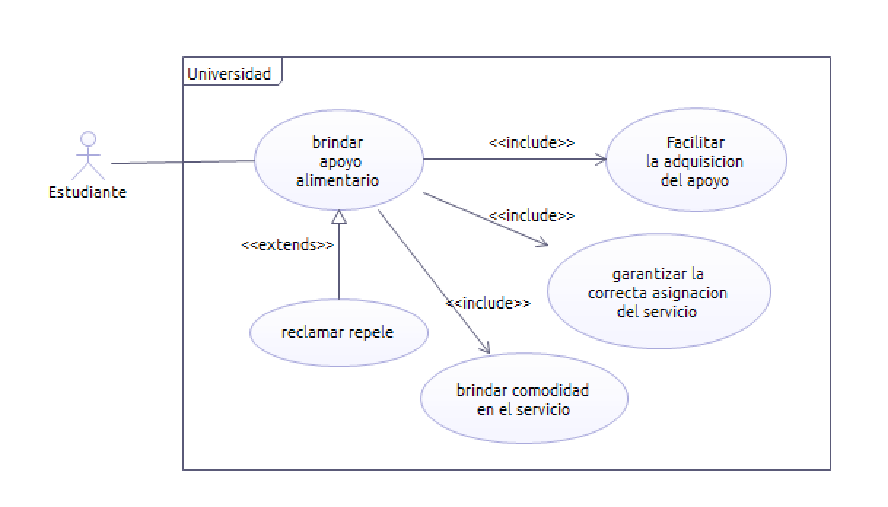
\includegraphics[width=0.8\linewidth]{parte2/imgs/CasosDeUso/caso1}
	\caption{Diagrama de caso de uso}
	\label{fig:diagramadecasodeuso}
\end{figure}

\section{Requerimientos de Casos de uso}

Los requerimientos de caso de uso entregan el plan de interacción entre el usuario y cada caso de uso: la descripción del caso de uso, los pasos para realizarse, las posibles fallas a las que puede incurrir, la prioridad y urgencia y comentarios acerca del mismo, todo para delimitar correctamente la relación usuario-aplicación
\begin{table}[H]
	\centering
	\caption{Caso de Uso CU-1}
	\label{my-label1}
	\begin{tabular}{|l|l|}
		\hline
		\textbf{Nombre}      & Brindar Apoyo Alimentario                                                                                                                                                   \\ \hline
		\textbf{Actores}     & Estudiantes                                                                                                                                                                 \\ \hline
		\textbf{Escenario}   &                                                                                                                                                                             \\ \hline
		\textbf{Primario}    & Brindar Apoyo Alimentario                                                                                                                                                   \\ \hline
		\textbf{Secundario}  & No coinciden Horarios                                                                                                                                                       \\ \hline
		\textbf{Excepciones} & \begin{tabular}[c]{@{}l@{}}Solicitud de Inscripción no aceptada, Estudiante no Registrado,\\ Se acabo el alimento, Ser retirado del beneficio por alguna falla\end{tabular} \\ \hline
	\end{tabular}
\end{table}

\begin{table}[H]
	\centering
	\caption{Caso de Uso CU-2}
	\label{my-label2}
	\begin{tabular}{|l|l|}
		\hline
		\textbf{Nombre}      & Reclamar Repele                                                                                                                                          \\ \hline
		\textbf{Actores}     & Estudiantes                                                                                                                                              \\ \hline
		\textbf{Escenario}   &                                                                                                                                                          \\ \hline
		\textbf{Primario}    & Reclamar Repele                                                                                                                                          \\ \hline
		\textbf{Secundario}  &                                                                                                                                                          \\ \hline
		\textbf{Excepciones} & \begin{tabular}[c]{@{}l@{}}No sobro alimento, Estudiante no Registrado, Ser retirado del beneficio,\\ La hora del reclamo no es la adecuada\end{tabular} \\ \hline
	\end{tabular}
\end{table}

\begin{table}[H]
	\centering
	\caption{Caso de Uso CU-3}
	\label{my-label3}
	\begin{tabular}{|l|l|}
		\hline
		\textbf{Nombre}      & Brindar Comodidad en el Servicio                                                                                                                                            \\ \hline
		\textbf{Actores}     & Administrativos, Estudiantes                                                                                                                                                \\ \hline
		\textbf{Escenario}   &                                                                                                                                                                             \\ \hline
		\textbf{Primario}    & Brindar Comodidad en el Servicio                                                                                                                                            \\ \hline
		\textbf{Secundario}  & Presentar Inscripción en la fechas no estipuladas                                                                                                                           \\ \hline
		\textbf{Excepciones} & \begin{tabular}[c]{@{}l@{}}Se presenta algún error en la Infreestructura, No se abríran convocatorias\\ No se cuentan con los espacios o horarios disponibles.\end{tabular} \\ \hline
	\end{tabular}
\end{table}

\begin{table}[H]
	\centering
	\caption{Casso de Uso CU-4}
	\label{my-label4}
	\begin{tabular}{|l|l|}
		\hline
		\textbf{Nombre}      & Garantizar Correcta Asignación del Servicio                                                                                                                                                                                       \\ \hline
		\textbf{Actores}     & Empleados y Administrativos encargados del apoyo                                                                                                                                                                                  \\ \hline
		\textbf{Escenario}   &                                                                                                                                                                                                                                   \\ \hline
		\textbf{Primario}    & Garantizar Correcta Asignación del Servicio                                                                                                                                                                                       \\ \hline
		\textbf{Secundario}  & \begin{tabular}[c]{@{}l@{}}Presentarse en las horas no adecuadas, Presentar alguna inconveniente\\ en un requerimiento del Apoyo\end{tabular}                                                                                     \\ \hline
		\textbf{Excepciones} & \begin{tabular}[c]{@{}l@{}}Fallos en la Infreestructura, Falla del Personal encargado de brindar\\ el servicio, Inconvenientes presentados tanto en espacios como\\ horarios habilitados para la entrega del servicio\end{tabular} \\ \hline
	\end{tabular}
\end{table}

\begin{table}[H]
	\centering
	\caption{Caso de Uso CU-5}
	\label{my-label5}
	\begin{tabular}{|l|l|}
		\hline
		\textbf{Nombre}      & Facilitar Adquisición del Apoyo                                                                                                                                                      \\ \hline
		\textbf{Actores}     & Administrativos, Personal encargado de brindar el servicio                                                                                                                           \\ \hline
		\textbf{Escenario}   &                                                                                                                                                                                      \\ \hline
		\textbf{Primario}    & Facilitar Adquisión del Apoyo                                                                                                                                                        \\ \hline
		\textbf{Secundario}  & Presentar alguna inconsistencia en la inscripción o documentos que soportan la misma,                                                                                                \\ \hline
		\textbf{Excepciones} & \begin{tabular}[c]{@{}l@{}}Fallos en la Infreestructura, No poder optar por el beneficio por falta de cupos,\\ No tener el puntaje necesarios para recibir el beneficio\end{tabular} \\ \hline
	\end{tabular}
\end{table}

\clearpage
% Please add the following required packages to your document preamble:
% \usepackage[table,xcdraw]{xcolor}
% If you use beamer only pass "xcolor=table" option, i.e. \documentclass[xcolor=table]{beamer}

